\documentclass[11pt]{article}
\usepackage[a4paper,margin=27mm]{geometry}
\usepackage[T1]{fontenc}
\usepackage[utf8]{inputenc}
\usepackage{lmodern}
\usepackage{amsmath,amssymb,amsthm,mathtools}
\usepackage{graphicx}
\usepackage{booktabs}
\usepackage{array}
\usepackage{xcolor}
\usepackage{microtype}
\usepackage{hyperref}
\hypersetup{colorlinks=true,linkcolor=blue!45!black,citecolor=blue!45!black,urlcolor=blue!55!black}

\newtheorem{theorem}{Theorem}[section]
\newtheorem{proposition}[theorem]{Proposition}
\newtheorem{corollary}[theorem]{Corollary}
\newtheorem{lemma}[theorem]{Lemma}
\newtheorem{remark}[theorem]{Remark}
\newcommand{\Fp}{\mathbf F_p}
\newcommand{\Q}{\mathbf Q}
\newcommand{\Z}{\mathbf Z}
\newcommand{\Res}{\operatorname{Res}}
\newcommand{\Norm}{\operatorname{N}}
\newcommand{\Var}{\operatorname{Var}}
\newcommand{\Disc}{\operatorname{Disc}}
\newcommand{\ord}{\operatorname{ord}}

\title{\textbf{Arithmetic Quantum Cat Maps:}\\
Exact Fourth-Moment Reductions, Cyclotomic Row Support,\\
and Heisenberg-Scale Trace Criteria}
\author{Maksim Churilov}
\date{Research draft --- 5 September 2026}

\begin{document}
\maketitle

\begin{abstract}
We develop exact arithmetic reductions for a fourth-moment problem arising in
quantum cat maps and isolate two logically separate closure problems before a
microscopic Bohigas--Giannoni--Schmit (BGS) statement can be attempted.  Let
$p$ be an odd prime, let $H\le\mathbf F_p^\times$ have odd prime order $K$, and
put
\[
c(h)=\frac{h+1}{h-1},\qquad A=c(H\setminus\{1\}).
\]
An exact pair-key reduction gives
\[
B(t)=O(t)+2(p-2)C_H(t)+(p-2)^2\mathbf 1_{t=0},
\]
and both nontrivial fourth-moment fluctuation layers are controlled by the
additive energy $E_+(A)$.  A source-exact subgroup-curve theorem yields
\[
E_+(A)<34K^{8/3}\qquad(100<K<p^{3/4}/3),
\]
while the corrected off/off elliptic analysis gives
\[
\Var_{t\ne0}O(t)\ll pE_+(A)+K^2p+K^4p^{1/2}+K^4.
\]

The pointwise arithmetic obstruction admits a sharper exact geometry.  A
fixed-product decomposition reduces non-forced excess to intersections of
special affine copies of the prime cyclotomic trace set.  Fixed-degree
subresultants in the maximal real cyclotomic field define an exact split-prime
order-three support $\Lambda'_K{}^{(3)}$; outside it,
\[
E_+(A)\le 11(K-1)(K-2).
\]
Bass's prime-conductor relations for cyclotomic units imply a complete
characteristic-zero affine-intercept classification: every intercept fibre has
cardinality at most two, and all double fibres are explicit.  Thus order-three
intersections are genuinely created by finite reduction.

For a general row ratio we replace the many-coefficient subresultant support by
one scalar shift resultant
\[
\mathcal R_{K,r}(Z)
 =\Res_T\!\left(P_1(T),R_r(\alpha_rT+\beta_r+Z)\right)
 =c_0+c_1Z+c_2Z^2+\cdots,
\]
whose order at $Z=0$ is exactly the row-intersection number.  Hence the event
$I\ge3$ is equivalent to simultaneous vanishing of $c_0,c_1,c_2$ modulo one
split prime ideal.  Individual intersections are also congruences between
explicit products of cyclotomic units.  For each fixed ratio, the supported
split primes satisfy
\[
\sum_{p\equiv1\,(K),\ I_r(p)\ge3}\log p=O(K^3).
\]

The inverse ratio $r=-1$ has additional structure.  If
$F(X)=P(\tau+X)$ and $x_i$ are its roots, then universally
\[
\Res_X(F(X),F(Z-X))
 =2^mF(Z/2)\,S(Z)^2,
\qquad
S(Z)=\prod_{i<j}(Z-x_i-x_j),
\]
with $m=(K-1)/2$.  At split primes the diagonal factor is a unit at $Z=0$, so
$I_{-1}=2\ord_0S$ and the order-three event is exactly
$S(0)=S'(0)=0$.  Writing
$F_Z(X)=F(X+Z/2)=E_Z(X^2)+XO_Z(X^2)$, we further prove
\[
S(Z)=\pm\Res_Y(E_Z,O_Z).
\]
Thus the inverse support is controlled by a half-degree resultant and its
translation derivative, computable without the degree-$m^2$ shift resultant.

A companion minimal-extension theorem uses Frobenius: if
$f=\ord_K(p)$ and the order-$K$ subgroup is placed in $\mathbf F_{p^f}$, every
non-forced collision orbit has size exactly $f$.  Together with the global
resultant budget this gives a density-one exact baseline for unrestricted
prime pairs $K\asymp X^\theta$, $p\asymp X$ for every fixed $\theta<1/3$;
it does not improve the split slice, where $f=1$.

Finally, partition-M\"obius inversion and Poisson summation give an exact
trace-to-local-statistics bridge.  Microscopic band-limited $k$-point
statistics require joint trace information at powers of order the matrix
dimension, the Heisenberg scale.  The missing spectral theorem is therefore a
weighted Heisenberg-scale trace comparison for the correct desymmetrized block,
plus a high-frequency tail estimate beyond band-limited tests.  No microscopic
BGS/GOE/COE universality theorem is claimed.
Separately, a centered arithmetic normal form controls the actual cosine-kicked
Pell propagator at its recurrence time. It gives a wrapped Gaussian law for
its $K$th power at quantum kick strength $\tau/\sqrt{2K}$, with an explicit
normalized Hilbert--Schmidt comparison error. This concerns a vanishing
classical perturbation and logarithmic recurrence times, not microscopic BGS.
Compact positive-Fourier tests further give a negative microscopic result:
bounded critical kick parameters exclude bounded clustering pair limits
under global mean-density unfolding of the full odd spectrum. The resulting
necessary larger-kick condition is not a sufficient universality criterion.
\end{abstract}

\section{Scope and evidence discipline}

Throughout the split finite-field part, $p$ is an odd prime and
$H\le\Fp^\times$ has odd prime order $K$.  Division is in $\Fp$.  Universal
claims are called exact only when the load-bearing derivation is present;
finite computations are certificates, regressions or falsifiers, never
substitutes for asymptotic proof.  Literature inputs are used only with their
hypotheses checked in the required regime.

The distinction between moment information and microscopic spectral statistics
is essential.  Arithmetic cat-map literature contains strong matrix-element and
quantum-ergodicity results \cite{KR2005,KRR2007,DJ2024,KORS2025,BS2026}, while
random-matrix universality is rigorous for special model classes such as mixing
quantum graphs under their own hypotheses \cite{PW2014,PW2015}.  None of these
results is silently transferred to the arithmetic family considered here.

\section{Exact pair-key geometry}

For $x,y\in\Fp\setminus\{0,1\}$ define
\begin{equation}\label{eq:keydef}
 u=\frac{x}{y},\qquad
 v=\frac{x-1}{y-1},\qquad
 d=x-y.
\end{equation}

\begin{proposition}[Pair-key bijection]\label{prop:key}
If $x\ne y$, then $u,v\in\Fp^\times\setminus\{1\}$, $u\ne v$, and
\begin{equation}\label{eq:inverse}
 y=\frac{1-v}{u-v},\qquad
 x=\frac{u(1-v)}{u-v},\qquad
 d=\frac{(u-1)(v-1)}{v-u}.
\end{equation}
Conversely every such $(u,v)$ gives a unique admissible off-diagonal pair.
The diagonal collapses to $(u,v,d)=(1,1,0)$ with multiplicity $p-2$.
\end{proposition}

\begin{proof}
The equations $x=uy$ and $x-1=v(y-1)$ give $(u-v)y=1-v$, hence
\eqref{eq:inverse}.  The diagonal statement is immediate.
\end{proof}

Under the subgroup constraints $u,v\in H$, there are exactly
$(K-1)(K-2)$ admissible off-diagonal ordered pairs.  If $O(t)$ denotes the
off/off contribution and
\[
C_H(t)=\#\left\{(u,v)\in(H\setminus\{1\})^2:
 u\ne v,\ \frac{(u-1)(v-1)}{v-u}=t\right\},
\]
then exact bookkeeping gives
\begin{equation}\label{eq:Bdecomp}
B(t)=O(t)+2(p-2)C_H(t)+(p-2)^2\mathbf1_{t=0}.
\end{equation}
The factor two is essential: diagonal/off and off/diagonal are distinct ordered
classes.  The total count is
\begin{equation}\label{eq:V4}
|V_4|=(K^2+1)p^2-(6K^2+3K)p+13K^2-3K.
\end{equation}
If $\Sigma_4(q)=\sum_tB(t)e_p(qt)$, $V=\sum_tB(t)$ and $Z=B(0)$, finite
Fourier orthogonality gives
\begin{equation}\label{eq:meanvar}
\mathbb E_{q\ne0}\Sigma_4(q)=\frac{pZ-V}{p-1},
\qquad
\Var_{q\ne0}\Sigma_4(q)=p\Var_{t\ne0}B(t).
\end{equation}
No probabilistic independence assumption enters this reduction.

\section{Cayley energy and the best uniform bound}

Put
\[
c(h)=\frac{h+1}{h-1},\qquad A=c(H\setminus\{1\}).
\]
For $u\ne v$,
\begin{equation}\label{eq:cayley}
\frac{(u-1)(v-1)}{v-u}=\frac{2}{c(u)-c(v)},
\qquad c(h^{-1})=-c(h).
\end{equation}
Thus $A=-A$ and the nonzero multiplicities of $C_H$ are additive-difference
multiplicities of $A$ up to the permutation $x\mapsto2/x$.  Hence
\begin{equation}\label{eq:energyCH}
\sum_tC_H(t)^2=E_+(A)-|A|^2,
\qquad
E_+(A)=\sum_xr_{A-A}(x)^2.
\end{equation}
Identity and central inversion force the nonzero baseline
\begin{equation}\label{eq:forced}
(K-1)(2K-5).
\end{equation}
For the unnormalized Fourier transform,
\begin{equation}\label{eq:centered}
E_+(A)=\frac{(K-1)^4}{p}
 +\frac1p\sum_{q\ne0}|\widehat{1_A}(q)|^4.
\end{equation}
The sharp pointwise target is therefore
\begin{equation}\label{eq:sharp-target}
E_+(A)=\frac{(K-1)^4}{p}+O(K^{2+o(1)}).
\end{equation}

For $r_A(t)=\#\{(a,b)\in A^2:a+b=t\}$, clearing Cayley denominators gives
\[
(2-t)xy+t(x+y)-(2+t)=0,
\]
an absolutely irreducible bidegree-$(1,1)$ curve in odd characteristic.

\begin{theorem}[Direct pointwise Cayley bound]\label{thm:direct}
If
\[
100<K<\frac13p^{3/4},
\]
then
\begin{equation}\label{eq:direct}
E_+(A)<34K^{8/3}.
\end{equation}
\end{theorem}

\begin{proof}
For $t\ne0,-2$, the source form of Vyugin--Makarychev's subgroup-curve theorem
\cite{VM2015,MV2019} gives $r_A(t)\le32K^{2/3}$ after its degree hypotheses are
checked on the displayed bilinear polynomial.  The exceptional fibres satisfy
$r_A(0)=K-1$ and $r_A(-2)\le K-1$.  Since
$\sum_tr_A(t)=(K-1)^2$,
\[
E_+(A)
\le2(K-1)^2+32K^{2/3}\sum_{t\ne0,-2}r_A(t)
<34K^{8/3}.
\]
\end{proof}

\section{Prime-order rigidity, square resultants and discriminants}

Let $\zeta=e^{2\pi i/K}$.  Then
\[
c(\zeta^a)=-i\cot\frac{\pi a}{K}.
\]
Chowla's prime-modulus cotangent independence \cite{Chowla1970,Wang1982}
identifies the characteristic-zero Cayley set with a rational cross-polytope.

\begin{theorem}[Prime-order additive rigidity]\label{thm:add-rigidity}
Every characteristic-zero equal-difference collision among
$\{c(\zeta^a):a\in\mathbf F_K^*\}$ is identity or central inversion-swap.
\end{theorem}

For every admissible cleared collision polynomial $P(X)$, direct algebra gives
$P(X)=(X-1)^3Q(X)$ and a reciprocal relation for $Q$.  Passing to the maximal
real subfield yields:

\begin{theorem}[Square-resultant theorem]\label{thm:square-res}
\begin{equation}\label{eq:square-res}
\Res(\Phi_K,P)=K^3M^2,\qquad M\in\Z.
\end{equation}
For a non-forced characteristic-zero collision, $M\ne0$.
\end{theorem}

The Fibonacci slice
\[
\Res(\Phi_K(X),X^2+3X+1)=F_K^2
\]
shows that individual collision resultants can be exponentially large.  At
$K=131$, $p=F_{131}$, a Lucas primality certificate and independent Python/C++
arbitrary-precision computations give exact nonzero Cayley excess $32$; this is
a finite certificate, not an asymptotic theorem.  The primitive-divisor input
for the associated rational model is from \cite{Yabuta2001}.

Let $S_K$ be the primitive squarefree nonzero-difference polynomial obtained
from the resultant of the characteristic-zero Cayley polynomial with its
translate.  Then for split primes
\begin{equation}\label{eq:disc-class}
\Delta_K(p)>0\iff p\mid\Disc(S_K),
\qquad
\Delta_K(p)\le4v_p(\Disc(S_K)).
\end{equation}
Ratio-orbit factorization and Dedekind-sum separation \cite{JRW2011} give the
exact global form
\begin{equation}\label{eq:global-fourth}
|\Disc(S_K)|
 =2^{(K-1)^4/4}K^{(K-1)(K^2-7)/4}J_K^4
\end{equation}
for an integer $J_K>0$.  Exact computations show that the residual logarithmic
mass genuinely remains $K^4$-scale, so \eqref{eq:global-fourth} is structural,
not a hidden proof of \eqref{eq:sharp-target}.

\section{Fixed-product rows and exact split support}

For one valid subgroup pair put $u=xy$, $s=x+y$.  Then
\begin{equation}\label{eq:rowparam}
c(x)+c(y)=\frac{2(u-1)}{u-s+1}.
\end{equation}
At fixed $u\ne1$ and nonzero parameter there is at most one unordered pair.
Let $I_K(p)$ be the maximum number of common parameters of two distinct product
rows.  The exact cross-row decomposition gives
\begin{equation}\label{eq:rowenergy}
\Delta_K(p)\le4I_K(p)(K-1)(K-2).
\end{equation}

Normalize a row pair to $(1,r)$ and set
\[
\tau=\zeta+\zeta^{-1},\qquad
\alpha_r=U_{r-1}(\tau/2),\qquad
\beta_r=-2U_{r-2}(\tau/2).
\]
The row equation is the affine trace relation
\begin{equation}\label{eq:affinetrace}
Y=\alpha_rX+\beta_r.
\end{equation}
Let $C_K(T)$ be the minimal polynomial of $\tau$ and set
\[
H_K(T)=(T-2)C_K(T).
\]
The two full row polynomials have one unique characteristic-zero common trace,
the invalid row trace.  Removing it produces fixed-degree source/target
cofactors over $\Z[\tau]$.  For every split embedding prime $\mathfrak q$,
\begin{equation}\label{eq:gcdcount}
\deg\gcd(P_{K,r},Q_{K,r}\bmod\mathfrak q)
 =I_{1,r}(\mathfrak q).
\end{equation}

Let the coefficient ideal of the first three fixed-degree subresultants
contract to $\Lambda_{K,r}^{(3)}\Z$.

\begin{theorem}[Exact real-trace order-three support]\label{thm:lambda}
For every split rational prime $p\equiv1\pmod K$,
\[
p\mid\Lambda_{K,r}^{(3)}
\]
if and only if some row pair in ratio class $[r]$ has at least three common
Cayley parameters.
\end{theorem}

\begin{proof}[Proof sketch]
The valid cofactors remain fixed-degree and squarefree after split reduction,
so \eqref{eq:gcdcount} is exact.  Brown--Traub's fixed-degree subresultant
criterion \cite{BT1971} identifies gcd degree at least three with vanishing of
the first three subresultants.  Their coefficient ideal records simultaneous
vanishing in one prime ideal; contraction to $\Z$ gives the rational-prime
statement.
\end{proof}

After removing factors $2,K$ and multiplying over ratio classes, write the
result as $\Lambda'_K{}^{(3)}$.  Then
\begin{equation}\label{eq:outside-support}
p\nmid\Lambda'_K{}^{(3)}
\Longrightarrow
I_K(p)\le2,
\quad
\Delta_K(p)\le8(K-1)(K-2),
\quad
E_+(A)\le11(K-1)(K-2).
\end{equation}
The older dehomogenized $D'/G'$ invariants remain valid only as one-way
obstructions because specialization can reduce leading degree at projective
infinity.

\section{Characteristic-zero affine-intercept rigidity}

Write
\[
t_a=\zeta^a+\zeta^{-a},\qquad
s_a=\zeta^a-\zeta^{-a},\qquad
\gamma_r(a,b)=t_b-\alpha_rt_a.
\]
Let $[a]$ denote the trace class $a\sim-a$, and put
$E_j=|1-\zeta^j|$, $1\le j\le m=(K-1)/2$.

\begin{lemma}[Prime-conductor multiplicative independence]\label{lem:bass}
The positive numbers $E_1,\ldots,E_m$ are multiplicatively independent.
\end{lemma}

\begin{proof}
Bass's prime-power theorem for the group generated by $1-\zeta^j$, modulo
torsion, gives a free $\Z$-basis represented by one Galois orbit modulo complex
conjugation \cite{Bass1966}.  Squaring any multiplicative relation among the
absolute values turns it into a relation in this torsion-free group, forcing all
exponents to vanish.
\end{proof}

Use the elementary identities
\begin{equation}\label{eq:absfacts}
|s_n|=E_{[2n]},\qquad
|t_x-t_y|=E_{[x-y]}E_{[x+y]}.
\end{equation}

\begin{theorem}[Trace-intercept fibre rigidity]\label{thm:intercept}
For every odd prime $K\ge7$ and every normalized ratio $r\ne1$, every fibre of
$([a],[b])\mapsto\gamma_r(a,b)$ has cardinality at most two.

If $r=-1$, a double fibre is only a swap.  If $r\ne\pm1$, every double fibre is,
up to signs and exchange,
\begin{equation}\label{eq:doublefibre}
([a],[a+1-r]),\qquad([a+2],[a+1+r]).
\end{equation}
\end{theorem}

\begin{proof}
Suppose two distinct pairs have the same intercept.  For $r\ne-1$,
\[
t_b-t_d=\alpha_r(t_a-t_c).
\]
Taking absolute values and applying \eqref{eq:absfacts} yields
\[
E_{[b-d]}E_{[b+d]}E_{[2]}
 =E_{[a-c]}E_{[a+c]}E_{[2r]}.
\]
Lemma~\ref{lem:bass} makes the multisets of folded indices equal.  Since
$[2r]\ne[2]$, one source difference must be $[2]$; after changing signs and
ordering take $c=a+2$.  The remaining two indices force the target classes in
\eqref{eq:doublefibre}.  The equality itself follows from
\[
t_{x+r}-t_{x-r}=s_rs_x,
\qquad
t_{a+2}-t_a=s_1s_{a+1}.
\]
A third point would form a triangle in the step-two quotient of the odd
$K$-cycle by $a\sim-a$; that quotient is a path.  For $r=-1$ the intercept is
$t_a+t_b$, and prime cyclotomic linear independence leaves only identity or
swap.
\end{proof}

The distinguished characteristic-zero row solution $([1],[r])$ is therefore
isolated.  This mechanism is related to cyclotomic-unit cross-ratio methods in
projective equivalence of roots of unity \cite{Fu2022}, but the affine theorem
above is proved directly in the prime-conductor setting.

\section{Cyclotomic-unit matching and a scalar shift resultant}

Put $u_n=s_n/s_1$.  For valid trace classes define
\begin{equation}\label{eq:WV}
W_r(b)=u_{(b+r)/2}u_{(b-r)/2},\qquad
V_r(a)=u_ru_{(a+1)/2}u_{(a-1)/2}.
\end{equation}
A direct difference factorization gives
\begin{equation}\label{eq:unitmatch}
\gamma_r(a,b)-\beta_r=s_1^2\bigl(W_r(b)-V_r(a)\bigr).
\end{equation}
Since $s_1$ is a unit away from $K$, every split row intersection is exactly a
congruence $W_r(b)\equiv V_r(a)\pmod{\mathfrak q}$ between explicit products
of cyclotomic units.

Let
\[
P_1(T)=\frac{H_K(T)}{T-t_1},\qquad
R_r(U)=\frac{H_K(U)}{U-t_r}
\]
and define the scalar shift resultant
\begin{equation}\label{eq:shiftres}
\mathcal R_{K,r}(Z)
 =\Res_T\!\left(P_1(T),R_r(\alpha_rT+\beta_r+Z)\right)
 =c_0+c_1Z+c_2Z^2+\cdots.
\end{equation}

\begin{theorem}[Scalar support identity]\label{thm:scalar-support}
For every split embedding prime $\mathfrak q$,
\begin{equation}\label{eq:ordshift}
\ord_{Z=0}(\mathcal R_{K,r}(Z)\bmod\mathfrak q)
 =I_{1,r}(\mathfrak q).
\end{equation}
Consequently
\[
I_{1,r}(\mathfrak q)\ge3
\iff
c_0\equiv c_1\equiv c_2\equiv0\pmod{\mathfrak q}.
\]
\end{theorem}

\begin{proof}
Over the split residue field the two valid trace polynomials factor linearly,
so the product formula gives
\[
\mathcal R_{K,r}(Z)
 =\prod_{[a]\ne[1]}\prod_{[b]\ne[r]}
   (Z+\alpha_rt_a+\beta_r-t_b).
\]
Each factor is linear in $Z$ and vanishes at zero exactly for one row
intersection.
\end{proof}

The ideal $(c_0,c_1,c_2)$ contracts to an integer
$\Omega_{K,r}^{(3)}$ with the same split rational-prime order-three support as
$\Lambda_{K,r}^{(3)}$.  Equality of the full integers is not asserted.
Moreover, the nonzero characteristic-zero constant coefficient gives the
per-ratio deterministic budget
\begin{equation}\label{eq:perratio}
\sum_{\substack{p\equiv1\,(K)\\I_r(p)\ge3}}\log p=O(K^3).
\end{equation}
Summing over $O(K)$ ratio classes recovers an $O(K^4)$ scale, so
\eqref{eq:perratio} is not a polynomial largest-prime theorem.

\section{Inverse reflection and the pair-sum square}

The ratio $r=-1$ has additional symmetry.  Here
\[
\alpha=-1,\qquad \beta=2\tau,
\qquad Q(T)=-P(2\tau-T).
\]
Set
\begin{equation}\label{eq:FEO}
F(X)=P(\tau+X)=E(X^2)+XO(X^2).
\end{equation}
The reflection reduction gives
\begin{equation}\label{eq:inverse-gcd}
I_{-1}(\mathfrak q)=2\deg\gcd(E,O\bmod\mathfrak q).
\end{equation}
Thus inverse-row intersections are automatically even.  A fixed-degree
half-size subresultant construction defines the exact split support integer
$\Xi_K$.

The scalar shift resultant admits a stronger universal factorization.

\begin{theorem}[Inverse pair-sum factorization]\label{thm:pairsum}
Let $x_1,\ldots,x_m$ be the roots of the monic polynomial $F$.  Define
\[
S(Z)=\prod_{i<j}(Z-x_i-x_j).
\]
Then $S\in\Z[\tau][Z]$ and
\begin{equation}\label{eq:pairsquare}
\Res_X(F(X),F(Z-X))=2^mF(Z/2)S(Z)^2.
\end{equation}
For every split embedding prime,
\begin{equation}\label{eq:inverse-order}
I_{-1}(\mathfrak q)=2\ord_{Z=0}(S(Z)\bmod\mathfrak q).
\end{equation}
Hence
\begin{equation}\label{eq:two-scalar}
I_{-1}(\mathfrak q)\ge3
\iff
S(0)\equiv S'(0)\equiv0\pmod{\mathfrak q}.
\end{equation}
\end{theorem}

\begin{proof}
The root-product formula gives
\[
\Res_X(F(X),F(Z-X))=\prod_{i,j}(Z-x_i-x_j).
\]
The diagonal ordered pairs give $2^mF(Z/2)$, and every unordered pair $i<j$
occurs twice.  The coefficients of $S$ are symmetric integral polynomials in
the roots.  At a split prime, $F(0)=P(\tau)=H'_K(\tau)$ is nonzero modulo every
embedding prime, so the diagonal factor is a unit at $Z=0$.  Combining with the
general shift-resultant identity gives \eqref{eq:inverse-order};
\eqref{eq:two-scalar} follows because the left side is even.
\end{proof}

Let $S(Z)=s_0+s_1Z+\cdots$ and let the ideal $(s_0,s_1)$ contract to
$\Theta_K\Z$.  Then $\Theta_K$, $\Xi_K$, and the inverse factor of
$\Lambda_{K,-1}^{(3)}$ have the same split rational-prime support; their
valuations need not agree.

\section{The pair-sum polynomial as a translated half-degree resultant}

The square root $S$ itself can be obtained without constructing the
degree-$m^2$ shift resultant.  Translate
\begin{equation}\label{eq:translatedF}
F_Z(X)=F(X+Z/2)=E_Z(X^2)+XO_Z(X^2).
\end{equation}

\begin{theorem}[Translated parity-resultant identity]\label{thm:translated-res}
There exists a convention-dependent sign $\varepsilon_m\in\{\pm1\}$ such that
\begin{equation}\label{eq:translated-res}
S(Z)=\varepsilon_m\Res_Y(E_Z(Y),O_Z(Y)).
\end{equation}
Consequently
\begin{align}
S(0)&=\varepsilon_m\Res_Y(E,O),\label{eq:s0res}\\
S'(0)&=\varepsilon_m
\left.\frac{d}{dZ}\Res_Y(E_Z,O_Z)\right|_{Z=0}.\label{eq:s1res}
\end{align}
The first-order deformation is
\begin{equation}\label{eq:deformation}
\left.\partial_ZE_Z\right|_0=\frac{O+2YO'}{2},
\qquad
\left.\partial_ZO_Z\right|_0=E'.
\end{equation}
\end{theorem}

\begin{proof}
The roots of $F_Z$ are $y_i=x_i-Z/2$.  Apply the constant pair-sum identity
from Theorem~\ref{thm:pairsum} to the monic polynomial $F_Z$.  Its unordered
pair-sum product at zero is
\[
\prod_{i<j}(-y_i-y_j)
 =\prod_{i<j}(Z-x_i-x_j)=S(Z).
\]
The even/odd decomposition \eqref{eq:translatedF} identifies this product,
up to the fixed resultant sign, with $\Res(E_Z,O_Z)$.  Differentiating
$F(X+Z/2)$ at $Z=0$ gives \eqref{eq:deformation}.
\end{proof}

Thus inverse order-three support is the simultaneous divisibility problem for a
half-degree resultant and its translation derivative.  In exact computation,
both scalars can be obtained in one Sylvester determinant over dual numbers
$\varepsilon^2=0$, reducing the determinant dimension to $O(K)$ rather than
materializing a degree-$m^2$ polynomial.

Exact Smith contractions give, after removing factors $2K$,
\[
\Theta'_7=1,\quad
\Theta'_{11}=1,\quad
\Theta'_{13}=5,\quad
\Theta'_{17}=1,\quad
\Theta'_{19}=37,\quad
\Theta'_{23}=47^2\cdot137.
\]
For comparison $\Xi'_{23}=47\cdot137$: split prime support agrees, valuations
differ.  The reference SymPy implementation reduces the $K=17$ computation
from roughly $51$ seconds for the full shift resultant to roughly $0.6$ seconds
for the translated half-degree route; at $K=23$ the latter remains on the
order of seconds, after which Smith normal form becomes the principal finite
algebra bottleneck.  These timings are reproducibility data, not asymptotic
complexity theorems.

The norm of the inverse constant shift coefficient also has the exact shape
\begin{equation}\label{eq:inverse-norm}
\left|\Norm(R_-(0))\right|
 =2^{m^2}K^m\left|\Norm(\Res(E,O))\right|^2,
\end{equation}
using $|\Norm(F(0))|=K^m$.  Hence every prime away from $2K$ occurs with even
valuation in this particular norm.  This explains part of the observed square
pattern but does not imply equality of the support integers.

\section{Global split-prime budget and minimal-extension Frobenius}

Simultaneous multiplication of collision exponent indices by
$a\in\mathbf F_K^\times$ acts freely on non-forced collision quadruples.  The
number of normalized scaling orbits is
\[
N_K=K^3-5K^2+6K+1.
\]
Combining the square-resultant theorem with $|\Res(\Phi_K,P)|\le12^{K-1}$
gives:

\begin{theorem}[Weighted split-prime budget]\label{thm:budget}
\begin{equation}\label{eq:budget}
\sum_{p\equiv1\,(K)}\Delta_K(p)\log p
\le N_K\bigl((K-1)\log12-3\log K\bigr).
\end{equation}
\end{theorem}

For prime $K\asymp X^\theta$ and split prime $p\asymp X$,
Bombieri--Vinogradov and PNT \cite{Bombieri1965,IK2004} imply
\[
\operatorname{average}\frac{\Delta_K(p)}{K^2}
 \ll_\theta X^{3\theta-1}
\]
for fixed $\theta<1/3$.  Integrality of the excess strengthens this to a
density-one exact baseline for fixed $\theta<1/5$:
\[
\Delta_K(p)=0,
\qquad
E_+(A)=3(K-1)(K-2)
\]
for asymptotically almost every split pair.

Now let $p\ne2,K$ be arbitrary and put
\[
f=\ord_K(p),\qquad q=p^f.
\]
In $\mathbf F_q$ the order-$K$ subgroup exists uniquely.

\begin{theorem}[Frobenius amplification]\label{thm:frob}
Every non-forced collision orbit under the $p$-power Frobenius has size exactly
$f$.  Hence
\[
f\mid\Delta_K^{\rm ext}(p).
\]
The weighted resultant budget and the discriminant classification extend to
all such rational primes in the minimal extension.
\end{theorem}

\begin{proof}
Frobenius multiplies every exponent by $p$ modulo $K$.  If a positive power
$d<f$ fixed a collision tuple, any nonzero coordinate would imply
$p^d\equiv1\pmod K$, contradicting the definition of $f$.  The resultant
argument is applied at one prime ideal over $p$; $p\ne K$ is unramified, so its
valuation on rational integers is the ordinary $p$-valuation.
\end{proof}

PNT, Brun--Titchmarsh and the scarcity of small multiplicative orders then give
a density-one exact baseline for unrestricted prime pairs
$K\asymp X^\theta$, $p\asymp X$ for every fixed $\theta<1/3$.  This mechanism
is absent on the split slice because there $f=1$.

\section{Full Cayley--Jacobi trace and corrected off/off geometry}

Let $S=H^\perp$ be the multiplicative-character annihilator and define the
normalized twisted-Jacobi matrix
\[
M_S(q)=\frac{e_p(-q/2)}{p-1}J_S(q).
\]
Character orthogonality gives the exact trace identity
\begin{equation}\label{eq:jacobi}
\widehat{1_A}(r)=K\operatorname{Tr}M_S(2r),
\end{equation}
and therefore
\begin{align}
\sum_q|\operatorname{Tr}M_S(q)|^2&=\frac{p(K-1)}{K^2},\label{eq:trace2}\\
\sum_q|\operatorname{Tr}M_S(q)|^4&=\frac{pE_+(A)}{K^4}.\label{eq:trace4}
\end{align}
The normalized fourth/second moment ratio tends to $3$ in the maintained split
double average below $\theta<1/3$.  This is a fourth-moment theorem, not a CLT.

The pure off/off family contains a coherent reducible fibre.  For generic
$\lambda=(h_1,h_2)$ it occurs at
\[
t_\lambda=\frac{2}{c(h_1)-c(h_2)}
\]
and has exactly $2p-8$ valid affine points.  After extracting the spike, Igusa
geometric monodromy \cite{BLV2009} and the Fouvry--Kowalski--Michel
trace-correlation argument \cite{FKM2013} give square-root quasi-orthogonality
between non-isomorphic geometric parameter classes.

\begin{theorem}[Corrected off/off variance]\label{thm:offoff}
\begin{equation}\label{eq:offoff}
\Var_{t\ne0}O(t)
\ll pE_+(A)+K^2p+K^4p^{1/2}+K^4,
\end{equation}
with an absolute implied constant.
\end{theorem}

Thus the off/off layer has collapsed onto the same pointwise Cayley-energy
bottleneck as the mixed layer.

\section{Exact trace-to-local-statistics bridge}

Let $U$ be an $N\times N$ unitary matrix with eigenvalues
$e^{2\pi i\theta_1},\ldots,e^{2\pi i\theta_N}$.  For a zero-sum integer tuple
$m_1+\cdots+m_k=0$, define
\[
D_U(m_1,\ldots,m_k)
 =\sum_{j_1,\ldots,j_k\ \mathrm{distinct}}
 e^{2\pi i\sum_{a=1}^km_a\theta_{j_a}}.
\]
For a set partition $\pi$ of $\{1,\ldots,k\}$, put
\[
\mu(\pi)=\prod_{B\in\pi}(-1)^{|B|-1}(|B|-1)!.
\]

\begin{theorem}[Factorial trace identity]\label{thm:factorial}
\begin{equation}\label{eq:factorial}
D_U(m_1,\ldots,m_k)
 =\sum_{\pi}\mu(\pi)
   \prod_{B\in\pi}
   \operatorname{Tr}U^{\sum_{a\in B}m_a}.
\end{equation}
\end{theorem}

This is M\"obius inversion on the partition lattice.  Let
$\phi\in\mathcal S(\mathbf R^{k-1})$ and periodize it at the mean-spacing scale.
Poisson summation gives the exact microscopic statistic
\begin{equation}\label{eq:trace-local}
C_{k,N}(U;\phi)
 =N^{-k}\sum_{m\in\Z^{k-1}}
  \widehat\phi(m/N)D_U(m_1,\ldots,m_k),
\end{equation}
where $m_k=-(m_1+\cdots+m_{k-1})$.  In particular,
\begin{equation}\label{eq:pair-local}
C_{2,N}(U;\phi)
 =N^{-2}\sum_{m\in\Z}\widehat\phi(m/N)
  \bigl(|\operatorname{Tr}U^m|^2-N\bigr).
\end{equation}
If $\widehat\phi$ has compact support, the relevant powers satisfy
$|m|=\Theta(N)$: microscopic local statistics probe the Heisenberg scale.

A weighted comparison of the quantities $D_U(m)$ with the matching random
matrix ensemble on this range is therefore sufficient for the corresponding
band-limited microscopic correlation theorem.  Arbitrary Schwartz tests
additionally require a uniform high-frequency tail bound.  This deterministic
Fourier bridge is exact; the required arithmetic/spectral joint-trace estimates
for the correct desymmetrized cat-map block remain open.

\section{Reproducibility and adversarial controls}

The maintained repository uses distinct failure modes:
\begin{itemize}
\item Python/SymPy regenerates exact resultants, discriminants, Smith
  contractions, finite-extension Frobenius checks, trace identities and the
  translated inverse-row support;
\item C++20 independently checks finite-field hot paths, arbitrary-precision
  witnesses and characteristic-zero trace-intercept fibres;
\item Lean 4 kernel-checks maintained finite certificates and falsifiers;
\item CI rebuilds all maintained code and recompiles this article; a separate
  workflow synchronizes the committed PDF from the TeX source.
\end{itemize}

The C++ trace-intercept verifier checks every normalized ratio through the
maintained quick range $K\le199$; a recorded extended run reaches prime
$K=809$, always with maximum fibre size two and the predicted double-fibre form.
The inverse translated-resultant verifier has exact Smith anchors through
$K=23$.  Representative prime-to-$2K$ contractions are
\[
\Theta'_{13}=5,\qquad
\Theta'_{19}=37,\qquad
\Theta'_{23}=47^2\cdot137.
\]
The independent reflection invariant gives
$\Xi'_{23}=47\cdot137$, confirming equal split prime support but different
valuation.  No integer equality is inferred.

Adversarial finite controls include $(K,p)=(29,728017)$ and $(31,1042903)$ with
$p>K^4$ but positive excess, disproving a bare ``$p>K^4$ implies baseline''
rule; $(K,p)=(41,2908049)$ has a row pair with two common parameters,
disproving $I_K(p)\le1$; and $(K,p)=(31,1303)$ has inverse-row intersection
size four.

\section{Fixed-map Pell blocks: a global Gaussian law and its rate}
\label{sec:pell}

Consider the fixed hyperbolic map and associated constants
\[
 T=\begin{pmatrix}3&2\\4&3\end{pmatrix},\qquad
 \alpha=1+\sqrt2,\qquad\lambda=\alpha^2.
\]
For each odd prime $K$, set $N+F\sqrt2=\alpha^K$, so that
$N^2-2F^2=-1$. The modulus $N$ may be composite. Put
$s=F^{-1}\pmod N$, $h=3+2s\pmod N$ and $q=-F\pmod N$.
Then $s^2=2$, and $h$ has exact order $K$ modulo each prime divisor of $N$.
In particular, $h^d-1$ is a unit for $0<d<K$, and $h^d+1$ is a unit for all $d$.

Use Weyl operators
\[
 \begin{gathered}
 (W(a,b)f)(x)=e_N(a(x-b/2))f(x-b),\qquad
 (S_hf)(x)=f(h^{-1}x),\\
 Q_j=\frac1K\sum_{t=0}^{K-1}e^{-2\pi ijt/K}S_h^t.
 \end{gathered}
\]
The explicit symplectic diagonalization in the maintained Pell note takes
the original cosine observable to the odd-sector blocks
\[
 A_j=\left.Q_j\{W(q,1)+W(q,1)^*\}Q_j\right|_{\rm odd},
 \qquad n=\frac{N-1}{2K},\qquad X_j=\sqrt{K/2}\,A_j.
\]
Each sector has dimension $n$, including at composite moduli.
The symmetrized observable preserves parity; an individual Weyl translation
need not do so. All claims here concern these observable blocks.

\begin{theorem}[Global Gaussian limit and rate]
For every fixed integer $r\ge1$, as $K$ tends to infinity through odd primes,
\[
 \sup_{0\le j<K}\left|n^{-1}\operatorname{Tr} X_j^{2r}-(2r-1)!!\right|
 =O_r(K^{-1})+O_r(K^{r+1}/N).
\]
For each fixed odd $m$ and all sufficiently large $K$,
\[
 \sup_j |n^{-1}\operatorname{Tr} X_j^m|
 \le 2^{m/2+1}K^{m/2+1}/(N-1).
\]
Thus the global empirical measures converge weakly to the variance-one
Gaussian, uniformly in the sequential choice of sector.
\end{theorem}

\begin{proof}
The fixed-point Weyl trace identity separates central reciprocal-zero words
from a remainder at most $2^{m/2+1}K^{m/2+1}/(N-1)$. The unit conditions
justify this estimate at composite $N$.

A modular reciprocal relation with $m$ signed terms can be rotated over its
largest cyclic gap. Its polynomial has degree at most $K-K/m$ and coefficient
$\ell^1$ norm at most $m$. If its value at $\lambda$ were nonzero, its algebraic
norm would be a nonzero multiple of $N^2$ but have absolute value at most
$m^2\lambda^{K-K/m}$. Since $N^2\asymp\lambda^K$, this is impossible for
fixed $m$ and large $K$. Hence the relation lifts to characteristic zero.
The minimal polynomial $x^2-6x+1$ takes value $-4$ at $1$, excluding odd
signed relations. The same norm argument shows that a gap exceeding
$2\log_\lambda m$ splits a relation. Bounded-width components then give
$O_r(K^{r-2})$ pinned nonpairable configurations, compared with $K^{r-1}$
paired configurations. Detailed component counting is in the Pell notes.

It remains to control crossing phases without a logarithmic loss.
Let $P_t$ be the Pell sequence, and let $\delta$ be the signed representative
of $d$ modulo $K$. Exactly,
\[
 z_d=e_N(q(h^d-h^{-d}))=e_N(-2P_{2\delta}).
\]
Writing $\delta=(K-1)/2-\ell$ for positive $\delta$ gives
\[
 \frac{P_{2\delta}}{N}
 =\frac{\lambda^{-\ell}}{\sqrt2\alpha}
 \frac{1-\lambda^{-2\delta}}{1-\lambda^{-K}}.
\]
Since $\alpha(1-\lambda^{-1})=2$, summing $|e^{it}-1|\le|t|$ yields
\[
 \sum_{d\bmod K}|z_d-1|
 \le \frac{2\sqrt2\pi}{1-\lambda^{-K}}<9.
\]
Each crossing label difference is uniform under pairing-label averaging,
even when one pair label is pinned. The product inequality for unit phases
therefore gives a mean error at most $9/K$ per crossing, without requiring
independence of different crossings. Repeated-label overcount and
nonpairable words contribute $O_r(K^{-1})$. The stated trace bounds follow.
Gaussian moment determinacy and higher even-moment bounds give weak convergence.
\end{proof}

\begin{theorem}[First fourth-moment correction]
For odd prime $K\ge11$, uniformly in $j$,
\[
 n^{-1}\operatorname{Tr} X_j^4=3-\frac{\gamma}{K}+O(K^3/N),
\]
where
\[
 \gamma=\frac32+2\sum_{\ell\ge0}
 \left[1-\cos\left(\frac{4\pi}{\sqrt2\alpha}\lambda^{-\ell}\right)\right]
 =5.61422069215\ldots.
\]
The following finite formula has an explicit remainder:
\[
 n^{-1}\operatorname{Tr} X_j^4=\frac{N}{N-1}\left(2+S_K-\frac{3}{2K}\right)+R_{4,j},
 \qquad |R_{4,j}|\le \frac{8K^3}{N-1},
\]
\[
 S_K=\frac1K\left(1+2\sum_{\delta=1}^{(K-1)/2}
                         \cos(4\pi P_{2\delta}/N)\right).
\]
\end{theorem}

\begin{proof}
Four-term reciprocal modular relations lift for $K\ge11$, since
$\lambda^{K/4}(1-\lambda^{-K})^2>64$. A lifted four-term relation pairs
because $\lambda>3$. Two pairings are noncrossing and one is crossing.
The six balanced all-equal sign words are counted twice; subtracting that
overcount gives $3/(2K)$. The noncentral fixed-point trace estimate gives
$R_{4,j}$. Reindexing the exact Pell ratio yields the cosine series.
The summed finite-argument error is $O(N^{-1})$ before division by $K$,
and the omitted cosine tail is $O(\lambda^{-K})$. With
$a=4\pi/(\sqrt2\alpha)$, the nonnegative tail after $J$ terms is at most
$a^2\lambda^{-2J}/(1-\lambda^{-2})$.
\end{proof}

\paragraph{Verification and scope.}
The independent orbit-matrix verifier includes nontrivial sectors and
$N=8119=23\cdot353$. Its matrix-power and eigenvalue moments are numerical
checks, not replacements for the proofs. The displayed decimal for $\gamma$ is now independently enclosed by
pure-integer interval arithmetic: Machin arctangent bounds, integer square
root, outward arithmetic, cosine Taylor remainders, and a geometric tail.
The separate matrix diagnostics still use floating-point arithmetic. Existing Lean certificates concern explicit finite word traces;
they do not formalize these general limit theorems. Priority remains unverified.
Neither this Gaussian global density nor an exact all-order trace formula
establishes local spacings or Heisenberg-scale universality for the propagator.

\IfFileExists{../assets/figures/pell_fourth_moment.png}{%
\begin{figure}[ht]
\centering
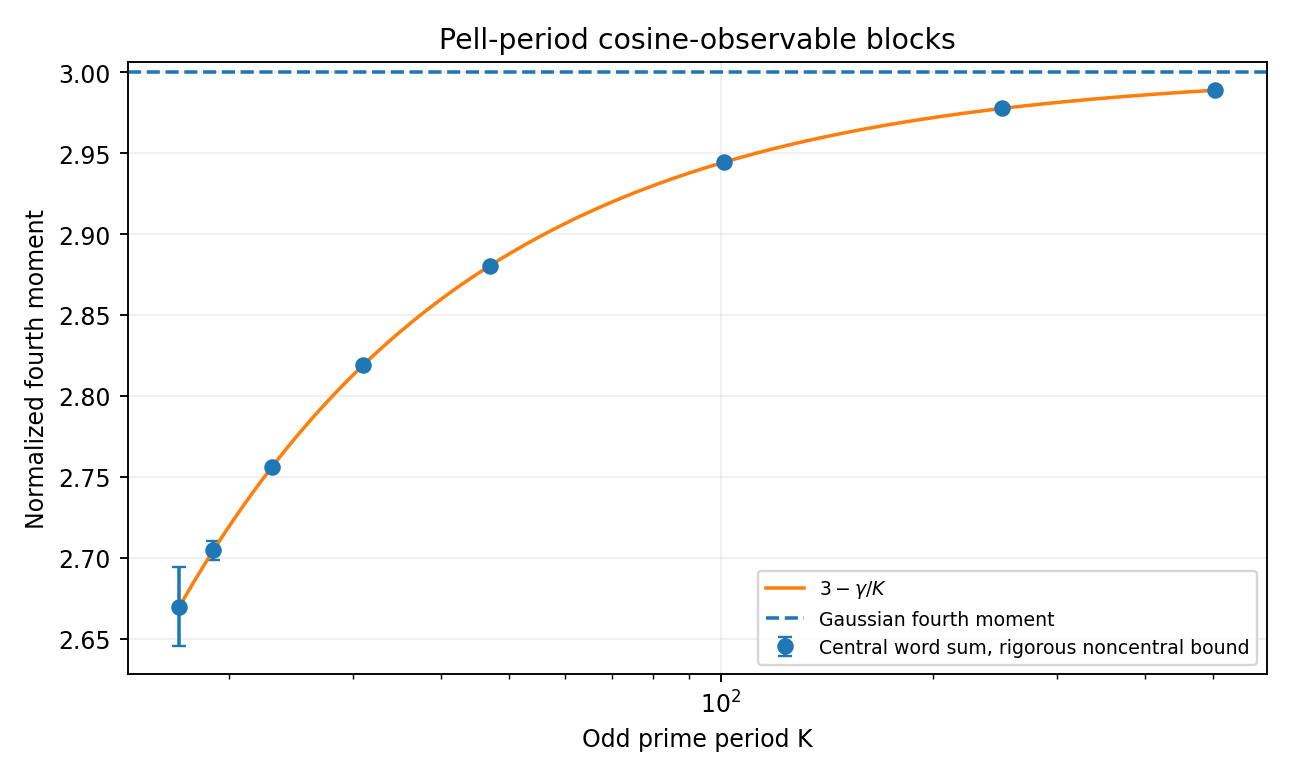
\includegraphics[width=.87\linewidth]{../assets/figures/pell_fourth_moment.png}
\caption{Central fourth-moment word sums with the explicit noncentral bound,
compared with $3-\gamma/K$. This is not a level-spacing plot.}
\end{figure}}{}

\section{An arithmetic normal form for the actual kicked propagator}
\label{sec:pell-floquet}
The Pell observable limit extends to an explicitly controlled spectral law
of the perturbed propagator at its recurrence time. This extension concerns
folded eigenphases, not microscopic BGS statistics. A self-contained proof,
including a direct odd-space Gaussian moment argument, is supplied in the
companion \emph{A resonance-scale spectral law for a deterministically kicked
Pell cat map} (\texttt{pell\_floquet\_normal\_form.pdf}).

Let $K\geq11$ be an odd prime, $N+F\sqrt2=(1+\sqrt2)^K$,
$h=3+2F^{-1}\pmod N$, $q=-F\pmod N$, and $d=(N-1)/2$. In the odd subspace set
\[
 U_0=S_h^{-1},\quad B=W(q,1)+W(q,1)^*,\quad
 U_\varepsilon=e^{i\varepsilon B}U_0,\quad
 \overline B=\frac1K\sum_{j=0}^{K-1}U_0^jBU_0^{-j}.
\]
This entire kicked family is unitarily equivalent to a fixed cosine
observable kicking the fixed map $T=\left(\begin{smallmatrix}3&2\\4&3\end{smallmatrix}\right)$.
The equivalence does not depend on primality of $N$.

\begin{theorem}[Finite normal form and critical recurrence law]
Put $B_j=U_0^jBU_0^{-j}$,
$c_j=(K-1-2j)/(2K)$, $G=\sum_jc_jB_j$ and
$V_\varepsilon=e^{-i\varepsilon G}$. For every real $\varepsilon$,
\[
 \left\|V_\varepsilon U_\varepsilon V_\varepsilon^*
               -e^{i\varepsilon\overline B}U_0\right\|_{2,-}
       \leq\frac{12\varepsilon^2}{\sqrt K},
 \qquad \|A\|_{2,-}^2=d^{-1}\operatorname{Tr}_{-}(A^*A).
\]
For each fixed real $\tau$, $\varepsilon=\tau/\sqrt{2K}$ and each integer $m$,
\[
 \frac1d\operatorname{Tr}_{-}U_\varepsilon^{mK}
       \longrightarrow e^{-m^2\tau^2/2}.
\]
Equivalently, the empirical eigenvalue measures of $U_\varepsilon^K$
converge to the wrapped normal law of $e^{i\tau Z}$, $Z\sim N(0,1)$.
\end{theorem}

\begin{proof}[Mechanism of the estimate]
The centered coefficients solve $G-U_0GU_0^*=B-\overline B$ exactly.
For $a_j=|e_N(q(h^j-h^{-j}))-1|$ and $\lambda=3+2\sqrt2$, Pell summation gives
\[
 \sum_j a_j<9,\qquad
 \sum_j|c_j|a_j\leq\frac{2\pi}{K(1-\lambda^{-K})}.
\]
Four-letter quadratic lifting makes all distinct-time signed pair sums
of Weyl indices different. Orthogonality in the \emph{full} Weyl space gives
\[
 \|[G,\overline B]\|_{2,N}^2
   =\frac4{K^4}\sum_{j=1}^{K-1}(K-j)j^2a_j^2\leq\frac9K.
\]
Also $\|[G,B]\|_{\rm op}<26/K$ and
$\|[B,\overline B]\|_{\rm op}<36/K$.
For Hermitian $A,D$, Duhamel's integral identity yields
\[
 \|e^{i\varepsilon A}e^{i\varepsilon D}
             -e^{i\varepsilon(A+D)}\|
 \leq\tfrac12\varepsilon^2\|[A,D]\|
\]
in either relevant unitarily invariant norm. Applied twice, this proves
the stated constant without requiring $\varepsilon\|G\|$ to be small.
Telescoping $mK$ powers and using $U_0^K=I$ leaves comparison error
$6|m|\tau^2/\sqrt K$ against
$d^{-1}\operatorname{Tr}_{-}\exp(im\tau X_K)$,
where $X_K=\sqrt{K/2}\,\overline B$. The Gaussian moment law for $X_K$
proves the limit. The comparison rate is not asserted as the total rate
of Gaussian characteristic-function convergence.
\end{proof}

\begin{corollary}[Subcritical folded phases]
If $\varepsilon_K\ne0$ and $\tau_K=\varepsilon_K\sqrt{2K}\to0$, then
\[
 \frac{\operatorname{Arg}(e^{iK\theta_\ell})}{\tau_K},
 \qquad e^{i\theta_\ell}\in\operatorname{Spec}(U_{\varepsilon_K}),
\]
have empirical measures converging in $W_2$ to $N(0,1)$.
No labelling into isolated old clusters is required. The proof bounds the
additional matching error by
$24|\tau_K|/\sqrt K+(6|\tau_K|/\pi)\sqrt{d^{-1}\operatorname{Tr}_{-}X_K^4}$.
\end{corollary}

The quantum kick at criticality tends to zero; its corresponding classical
strength is of order $1/(N\sqrt K)$. The recurrence time $K\asymp\log N$
is much shorter than the Heisenberg scale $d$. These statements do not
establish local spacing universality or the fixed-classical-perturbation
BGS conjecture. Priority for the specific arithmetic construction remains
unverified. Independent C++ and Python representations, finite Lean kernels,
and exact-versus-sampled numerical provenance are maintained separately.


\subsection{A compact-test obstruction to microscopic pair limits}
The recurrence trace law has a negative microscopic consequence even though
positive universality would require more information. Measure eigenphases
in turns, $e^{2\pi i x_a}$, and define
\[
 C_d(U;\phi)=\frac1d\sum_{a\ne b}\sum_{n\in\mathbb Z}
                  \phi(d(x_a-x_b+n)),\qquad
 \phi_L(s)=\frac1L(1-|s|/L)_+.
\]
This is the globally unfolded full odd spectrum, retaining multiplicities.
Since $\widehat\phi_L(u)=\operatorname{sinc}^2(Lu)\geq0$, where
$\operatorname{sinc}(v)=\sin(\pi v)/(\pi v)$, the exact Fourier formula
\[
 C_d(U;\phi_L)=d^{-2}\sum_{t\in\mathbb Z}
       \widehat\phi_L(t/d)(|\operatorname{Tr}U^t|^2-d)
\]
implies, for $d>L$ and every fixed $M$,
\[
 C_d(U;\phi_L)\geq 1-\frac1L+
 2\sum_{m=1}^M\operatorname{sinc}^2(LmK/d)
                 |d^{-1}\operatorname{Tr}U^{mK}|^2.
\]
No tail estimate is required: all omitted squared-trace terms are nonnegative.

\begin{theorem}[Necessary escape from the critical recurrence regime]
Suppose $\tau_K=\varepsilon_K\sqrt{2K}\to\tau\ne0$ is finite. Then
\[
 \liminf_K C_d(U_{\varepsilon_K};\phi_L)
    \geq\Theta(\tau)-1/L,\qquad
 \Theta(\tau)=\sum_{m\in\mathbb Z}e^{-m^2\tau^2}>1.
\]
If $N_L(y)$ counts levels in a uniformly translated interval of unfolded
length $L$, then
\[
 \liminf_K\operatorname{Var}_y N_L\geq L^2(\Theta(\tau)-1).
\]
If $\tau_K\to0$, the fixed-$L$ pair statistic diverges to infinity.
Consequently a globally unfolded pair limit with a bounded density tending
to $1$ at large separation requires $|\varepsilon_K|\sqrt K\to\infty$.
\end{theorem}

\begin{proof}
The trace limit is stable under $\tau_K\to\tau$ by the uniform second
moment of $X_K$. First take the lower limit at fixed $M,L$ above, using
$K/d\to0$, then let $M\to\infty$. For $\tau=0$ every retained trace has
limiting absolute value $1$, so the lower bound is unbounded in $M$.
Interval overlap gives exactly
$\operatorname{Var}N_L=L^2(C_d-1)+L$.
If the limiting pair density were bounded and satisfied $\rho(s)\to1$,
then its triangular average
$\int_{-1}^1(1-|u|)\rho(Lu)\,du$ would tend to $1$ as $L\to\infty$,
contradicting the lower bound. Any bounded subsequence of $\tau_K$ contains
a convergent subsequence, proving the necessary escape condition.
\end{proof}

The sine-kernel and Poisson pair laws are explicitly excluded: at
$L=e^{\tau^2}$, even the first resonance gives a limiting lower bound
$1+e^{-\tau^2}$, while both target averages are at most $1$. The standard
GOE bulk pair density is bounded and tends to $1$, so the general criterion
also excludes it. The companion checks this property directly from the
Brezin--Hikami formula, equation (181), arXiv:math-ph/0208001.
The continuous compact test may be replaced by a smooth compact
positive-definite autocorrelation; no unproved Schwartz-tail control is used.
This obstruction does not address density-adapted re-unfolding, further
symmetry sectors, or a fixed nonzero classical kick. It does not assert
that the necessary larger-kick condition is sufficient for BGS.


\section{Remaining frontier}

The arithmetic fourth-moment chain is now
\[
\begin{gathered}
\boxed{\text{common split divisors of small cyclotomic scalar systems}}
\\ \downarrow \\
\boxed{\text{pointwise centered Cayley energy}}
\\ \downarrow \\
\boxed{\text{complete fourth-moment control}}.
\end{gathered}
\]
For general ratios the order-three event is encoded by three scalar shift
coefficients; for the inverse ratio it reduces further to a half-degree
resultant and its translation derivative.  The existing per-ratio
$O(K^3)$ logarithmic mass does not bound the largest supported split prime
polynomially.  A sufficient remaining target is, for example,
\[
P^+_{\rm split}(\Lambda'_K{}^{(3)})\le K^{4+o(1)},
\]
or an equivalent theorem for the scalar support systems.  The high-value next
step is a uniform common-divisor/Bezout theorem, not another individual height
estimate.

The microscopic spectral chain is independently
\[
\begin{gathered}
\boxed{\text{Heisenberg-scale desymmetrized joint traces}}
\\ \downarrow \\
\boxed{\text{band-limited microscopic RMT correlations}}
\\ \downarrow \\
\boxed{\text{high-frequency tail control}}
\\ \downarrow \\
\boxed{\text{full microscopic BGS/RMT}}.
\end{gathered}
\]
The Fourier arrow is exact by \eqref{eq:factorial}--\eqref{eq:trace-local}; the
joint-trace estimate itself is open.  Fixed powers, finitely many moments, or
even a completed fourth-moment theorem cannot be promoted to microscopic BGS.

\section{Conclusion}

The fourth-moment problem has been reduced to a progressively smaller
arithmetic obstruction.  Fixed-product rows give an exact order-three split
support.  Prime-conductor cyclotomic-unit rigidity closes the corresponding
characteristic-zero fibre problem.  A scalar shift resultant compresses the
general finite event to three coefficients, while the inverse row admits an
additional perfect-square factorization that reduces the event to two
half-degree scalar quantities: a resultant and its translation derivative.
These reductions are exact and specialization-safe, but they do not yet supply
a polynomial largest-split-prime theorem.

Frobenius amplification yields a complementary density-one exact theorem over
minimal finite extensions while correctly leaving the split slice unchanged.
On the spectral side, the exact partition-M\"obius/Poisson identity identifies
Heisenberg-scale joint traces as the missing input for microscopic
correlations.  Full BGS/GOE/COE universality remains open.


\section{A second-order scale for a coboundary kick}
Let $A=B_{(1,0)}$, $D=U_0AU_0^*=B_{(3,4)}$ and
$V_\varepsilon=e^{i\varepsilon(A-D)}U_0$ in the same odd Pell quantization.
For $s_N=\sin(4\pi/N)$ and $t_K=2\varepsilon_K^2s_N\sqrt K$, the
companion proof establishes
\[
 t_K\longrightarrow t<\infty
 \quad\Longrightarrow\quad
 \frac{1}{d_N}\operatorname{Tr}_{-}V_{\varepsilon_K}^{mK}
       \longrightarrow e^{-m^2t^2/2}
 \qquad(m\in\mathbb Z).
\]
The resulting critical quantum scale is
$|\varepsilon_K|\asymp\sqrt N K^{-1/4}$, for this different fixed Fourier
observable. Its classical action amplitude is still proportional to
$\varepsilon_K/N$ and tends to zero.

The finite second-order comparison is
\[
 \left\|e^{-i\varepsilon A}V_\varepsilon e^{i\varepsilon A}
          -e^{i\varepsilon^2s_N C}U_0\right\|_{\rm op}
 \leq \frac{64}{3}|\varepsilon|^3s_N^2,
 \qquad C=B_{(2,4)}-B_{(4,4)}.
\]
It holds without requiring $|\varepsilon|\|A\|$ small. For the two
species generated by $C$, the structural identity
$T((4,4)-(2,4))=(4,4)+(2,4)$ prevents a false no-collision argument.
The exact replacement is a multiplicity-two theorem: for $K\geq11$ there
are $4K$ double distinct-time signed-pair keys and $8K(K-2)$ single keys.
This gives the Hilbert--Schmidt normal form needed for the spectral limit.

Compact nonnegative Fourier tests imply that bounded
$|\varepsilon_K|K^{1/4}/\sqrt N$ obstructs a bounded globally unfolded
pair density tending to one at large separation. In the subcritical regime,
nearest-neighbour spacings collapse to a point mass at zero and close-pair
counts diverge. These are negative microscopic conclusions for the specified
shrinking-classical-kick family, not a fixed-system BGS counterexample or a
positive universality theorem.

Residual perturbations and their second-order commutator are established in
Prosen and Znidaric, Phys. Rev. Lett. 94 (2005), 044101. The project does not
claim to originate that mechanism. The complete derivation and priority
boundary are maintained in
\texttt{mathematics/pell\_coboundary\_resonance.md} and its companion PDF.
General analytic arguments are not claimed to be fully formalized in Lean.

The generated observable also admits an exact finite fourth-moment formula.
For $X_K=(\sqrt K/2)\overline C$, the full-space and odd-space estimates are
\[
 \mu_{4,N}=3-\frac{\gamma_C}{K}+O\!\left(\frac1{KN}\right),
 \qquad
 \mu_{4,-}=3-\frac{\gamma_C}{K}+O\!\left(\frac{K^2}{N}\right),
\]
where $\gamma_C=4.178502650021\ldots$.
The closed formula and its separate parity-error budget are proved in the
companion article and checked independently against Weyl convolution.
High-precision decimals are not interval certificates.


\begin{thebibliography}{99}

\bibitem{KR2005}
P.~Kurlberg and Z.~Rudnick,
\emph{On the distribution of matrix elements for the quantum cat map},
Ann. of Math. \textbf{161} (2005), 489--507,
doi:10.4007/annals.2005.161.489.

\bibitem{KRR2007}
P.~Kurlberg, L.~Rosenzweig and Z.~Rudnick,
\emph{Matrix elements for the quantum cat map: fluctuations in short windows},
arXiv:math/0701685 (2007).

\bibitem{DJ2024}
S.~Dyatlov and M.~J\'ez\'equel,
\emph{Semiclassical Measures for Higher-Dimensional Quantum Cat Maps},
Ann. Henri Poincar\'e \textbf{25} (2024), 1545--1605,
doi:10.1007/s00023-023-01309-x.

\bibitem{KORS2025}
P.~Kurlberg, A.~Ostafe, Z.~Rudnick and I.~E.~Shparlinski,
\emph{On Quantum Ergodicity for Higher Dimensional Cat Maps},
Commun. Math. Phys. \textbf{406} (2025), 174,
doi:10.1007/s00220-025-05350-1.

\bibitem{BS2026}
S.~Bhakta and I.~E.~Shparlinski,
\emph{On quantum ergodicity for higher-dimensional cat maps modulo prime powers},
Bull. London Math. Soc. \textbf{58} (2026),
doi:10.1112/blms.70300.

\bibitem{PW2014}
Z.~Pluha\v r and H.~A.~Weidenm\"uller,
\emph{Universal Quantum Graphs},
Phys. Rev. Lett. \textbf{112} (2014), 144102,
doi:10.1103/PhysRevLett.112.144102.

\bibitem{PW2015}
Z.~Pluha\v r and H.~A.~Weidenm\"uller,
\emph{Quantum graphs and random-matrix theory},
J. Phys. A \textbf{48} (2015), 275102,
doi:10.1088/1751-8113/48/27/275102.

\bibitem{Chowla1970}
S.~Chowla,
\emph{The nonexistence of nontrivial linear relations between the roots of a certain irreducible equation},
J. Number Theory \textbf{2} (1970), 120--123,
doi:10.1016/0022-314X(70)90012-0.

\bibitem{Wang1982}
K.~Wang,
\emph{On a theorem of S. Chowla},
J. Number Theory \textbf{15} (1982), 1--4,
doi:10.1016/0022-314X(82)90078-6.

\bibitem{Bass1966}
H.~Bass,
\emph{Generators and Relations for Cyclotomic Units},
Nagoya Math. J. \textbf{27} (1966), 401--407,
doi:10.1017/S0027763000026258.

\bibitem{Fu2022}
H.~Fu,
\emph{Projective Equivalence for the Roots of Unity},
J. Algebraic Combin. \textbf{56} (2022), 823--871,
arXiv:1905.01510.

\bibitem{Yabuta2001}
M.~Yabuta,
\emph{A Simple Proof of Carmichael's Theorem on Primitive Divisors},
Fibonacci Quart. \textbf{39} (2001), 439--443,
doi:10.1080/00150517.2001.12428701.

\bibitem{VM2015}
I.~V.~Vyugin and S.~Makarychev,
\emph{Solutions of polynomial equation over $\mathbf F_p$ and new bounds of additive energy},
arXiv:1504.01354v2 (2015).

\bibitem{MV2019}
S.~Makarychev and I.~Vyugin,
\emph{Solutions of Polynomial Equations in Subgroups of $\mathbf F_p^*$},
Arnold Math. J. \textbf{5} (2019), 105--121,
doi:10.1007/s40598-019-00112-z.

\bibitem{JRW2011}
S.~Jabuka, S.~Robins and X.~Wang,
\emph{When are two Dedekind sums equal?},
Int. J. Number Theory \textbf{7} (2011), 2197--2203,
arXiv:1103.0370.

\bibitem{BT1971}
W.~S.~Brown and J.~F.~Traub,
\emph{On Euclid's Algorithm and the Theory of Subresultants},
J. ACM \textbf{18} (1971), 505--514,
doi:10.1145/321662.321665.

\bibitem{Bombieri1965}
E.~Bombieri,
\emph{On the large sieve},
Mathematika \textbf{12} (1965), 201--225,
doi:10.1112/S0025579300005313.

\bibitem{IK2004}
H.~Iwaniec and E.~Kowalski,
\emph{Analytic Number Theory},
AMS Colloquium Publications \textbf{53}, 2004,
doi:10.1090/coll/053.

\bibitem{FKM2013}
\'E.~Fouvry, E.~Kowalski and P.~Michel,
\emph{Counting sheaves using spherical codes},
Math. Res. Lett. \textbf{20} (2013), 305--323,
doi:10.4310/MRL.2013.V20.N2.A8,
arXiv:1210.0851.

\bibitem{BLV2009}
A.~Bandini, I.~Longhi and S.~Vigni,
\emph{Torsion points on elliptic curves over function fields and a theorem of Igusa},
Expo. Math. \textbf{27} (2009), 175--209,
doi:10.1016/j.exmath.2008.06.001,
arXiv:0804.1425.

\end{thebibliography}

\end{document}
